% !TEX program = pdflatex
% Compile from this folder:  pdflatex BO-Jira-Sheets-Documentation.tex   (run it twice for the table of contents)
\documentclass[11pt,a4paper]{article}

\usepackage[utf8]{inputenc}
\usepackage[T1]{fontenc}
\usepackage{lmodern}
\usepackage[a4paper,margin=2.4cm,top=2.8cm,bottom=2.4cm]{geometry}
\usepackage{xcolor}
\usepackage{graphicx}
\usepackage{tikz}
\usetikzlibrary{arrows.meta,positioning,calc,shapes.geometric,fit}
\usepackage{tcolorbox}
\tcbuselibrary{breakable,skins}
\usepackage{booktabs}
\usepackage{longtable}
\usepackage{tabularx}
\usepackage{array}
\usepackage{enumitem}
\usepackage{fancyhdr}
\usepackage{listings}
\usepackage{titlesec}
\usepackage{setspace}
\usepackage[hidelinks]{hyperref}
\usepackage{xurl}
\usepackage{amssymb}
\usepackage{needspace}

\graphicspath{{./}}

% ---------------------------------------------------------------- colours
\definecolor{navy}{HTML}{1B1F3B}
\definecolor{accent}{HTML}{2A9D8F}
\definecolor{soft}{HTML}{EEF4F3}
\definecolor{sheetgreen}{HTML}{B7E1CD}
\definecolor{sheetyellow}{HTML}{FCE8B2}
\definecolor{sheetred}{HTML}{F4C7C3}
\definecolor{sheetblue}{HTML}{C9DAF8}
\definecolor{sheetgrey}{HTML}{E8EAED}
\definecolor{sheetpurple}{HTML}{E1D5F0}
\definecolor{codebg}{HTML}{F6F8FA}

\hypersetup{pdftitle={BO Team Jira to Google Sheets Automation},pdfauthor={Mohamed Magdy}}

% ---------------------------------------------------------------- helpers
\newcommand{\code}[1]{\texttt{#1}}
\newcommand{\tab}[1]{\textbf{#1}}
\newcolumntype{L}{>{\raggedright\arraybackslash}X}
\newcommand{\swatch}[1]{\colorbox{#1}{\rule{0pt}{1.6ex}\hspace{1.4em}}}

\newtcolorbox{note}[1][Note]{enhanced,breakable,colback=soft,colframe=accent,coltitle=white,
  fonttitle=\bfseries,title=#1,boxrule=0.6pt,arc=2pt,left=6pt,right=6pt,top=4pt,bottom=4pt}
\newtcolorbox{warning}[1][Important]{enhanced,breakable,colback=sheetyellow!40,colframe=orange!80!black,
  coltitle=white,fonttitle=\bfseries,title=#1,boxrule=0.6pt,arc=2pt,left=6pt,right=6pt,top=4pt,bottom=4pt}

\lstset{basicstyle=\ttfamily\footnotesize,backgroundcolor=\color{codebg},frame=single,
  rulecolor=\color{black!20},breaklines=true,columns=fullflexible,keepspaces=true,
  showstringspaces=false,xleftmargin=2pt,xrightmargin=2pt,aboveskip=8pt,belowskip=8pt}

\titleformat{\section}{\Large\bfseries\color{navy}}{\thesection}{0.8em}{}[\vspace{-0.6em}\textcolor{accent}{\rule{\linewidth}{0.8pt}}]
\titleformat{\subsection}{\large\bfseries\color{navy}}{\thesubsection}{0.8em}{}
\titleformat{\subsubsection}{\normalsize\bfseries\color{accent!80!black}}{\thesubsubsection}{0.8em}{}
% keep a heading together with the text that follows it
\let\oldsection\section
\renewcommand{\section}{\needspace{12\baselineskip}\oldsection}
\let\oldsubsection\subsection
\renewcommand{\subsection}{\needspace{7\baselineskip}\oldsubsection}
\setlist{itemsep=2pt,topsep=4pt}
\setstretch{1.08}
\renewcommand{\arraystretch}{1.25}

% ---------------------------------------------------------------- header / footer
\pagestyle{fancy}
\fancyhf{}
\renewcommand{\headrulewidth}{0.4pt}
\fancyhead[L]{\raisebox{-0.35\height}{
\includegraphics[height=0.55cm]{logo-dark.png}}}
\fancyhead[R]{\small\color{navy}BO Team: Jira to Google Sheets Automation}
\fancyfoot[L]{\small\color{black!60}Prepared by Mohamed Magdy}
\fancyfoot[R]{\small\color{black!60}Page \thepage}
\setlength{\headheight}{16pt}

\begin{document}

% ================================================================ COVER PAGE
\begin{titlepage}
\thispagestyle{empty}
\begin{tikzpicture}[remember picture,overlay]
  \fill[navy] (current page.north west) rectangle ([yshift=-10.5cm]current page.north east);
  \fill[accent] ([yshift=-10.5cm]current page.north west) rectangle ([yshift=-10.75cm]current page.north east);
  \node at ([yshift=-5.2cm]current page.north) {
\includegraphics[width=10.5cm]{logo-light.png}};
\end{tikzpicture}

\vspace*{9.2cm}
\begin{center}
  {\fontsize{26}{32}\selectfont\bfseries\color{navy} BO Team:\\[2pt] Jira to Google Sheets Automation}\\[1.1cm]
  {\Large\color{accent!80!black} Technical and User Documentation}\\[0.5cm]
  {\large How the sheets are built, how to read them, and how to keep them running}
\end{center}

\vfill
\begin{center}
  \begin{tabular}{rl}
    \textbf{Created by} & Mohamed Magdy \\
    \textbf{Company}    & Connect Money \\
    \textbf{Team}       & Back Office (BO), Jira project \code{L1} \\
    \textbf{Version}    & 1.1 \\
    \textbf{Date}       & 5 October 2026 \\
  \end{tabular}
\end{center}
\vspace{0.6cm}
\end{titlepage}

\setcounter{page}{2}
\tableofcontents
\clearpage

% ================================================================ 1 INTRODUCTION
\section{Introduction}

\subsection{What this system does}
The BO team receives its work as Jira tickets in the project \textbf{L1 Support (BO)} (key \code{L1}). Before this
project, the team tracked those tickets by hand in Google Sheets. This system copies the tickets from Jira into two
Google Sheets \emph{automatically}, keeps them up to date during the day and night, and adds the numbers the team lead
needs: backlog per contact type, tickets per team and per person, time spent in each status, and productivity.

In one sentence: \textbf{Jira stays the source of truth; the two Google Sheets are a live, easy-to-read, easy-to-edit
view of it.}

\subsection{The two sheets}
\begin{tabularx}{\linewidth}{@{}l L@{}}
\toprule
\textbf{Sheet} & \textbf{Purpose} \\
\midrule
\tab{BO Tickets (Auto)} & New work. Shows the tickets that are still waiting to be picked up (Jira status
\emph{To Do} or \emph{Clients To Do}), split by team (MDB, Installment, Product, Others), with a backlog table and a
productivity summary. \\
\tab{In Progress} & Work in flight. Shows the tickets that the team is working on, tickets waiting for the
customer, and each person's workload and results. \\
\bottomrule
\end{tabularx}

\subsection{Who should read which part}
\begin{tabularx}{\linewidth}{@{}l L l@{}}
\toprule
\textbf{Reader} & \textbf{What you need} & \textbf{Chapters} \\
\midrule
BO team member & How to read the sheets and use the dropdowns & 4, 5 \\
Team lead / manager & What each number means and how reliable it is & 4, 5, 9, 10 \\
Maintainer & How it runs, how to change it, how to fix it & 2, 6, 7, 8, 9 \\
Anyone new & Terms used in this document & Appendix A \\
\bottomrule
\end{tabularx}

\subsection{Conventions}
Names of tabs, columns, and dropdown values are written in \textbf{bold}. File names, settings, and commands are
written in \code{typewriter font}. All times are in \textbf{Cairo time} (Africa/Cairo) unless stated otherwise.

% ================================================================ 2 ARCHITECTURE
\section{System at a Glance}

\subsection{The moving parts}
\begin{figure}[h]
\centering
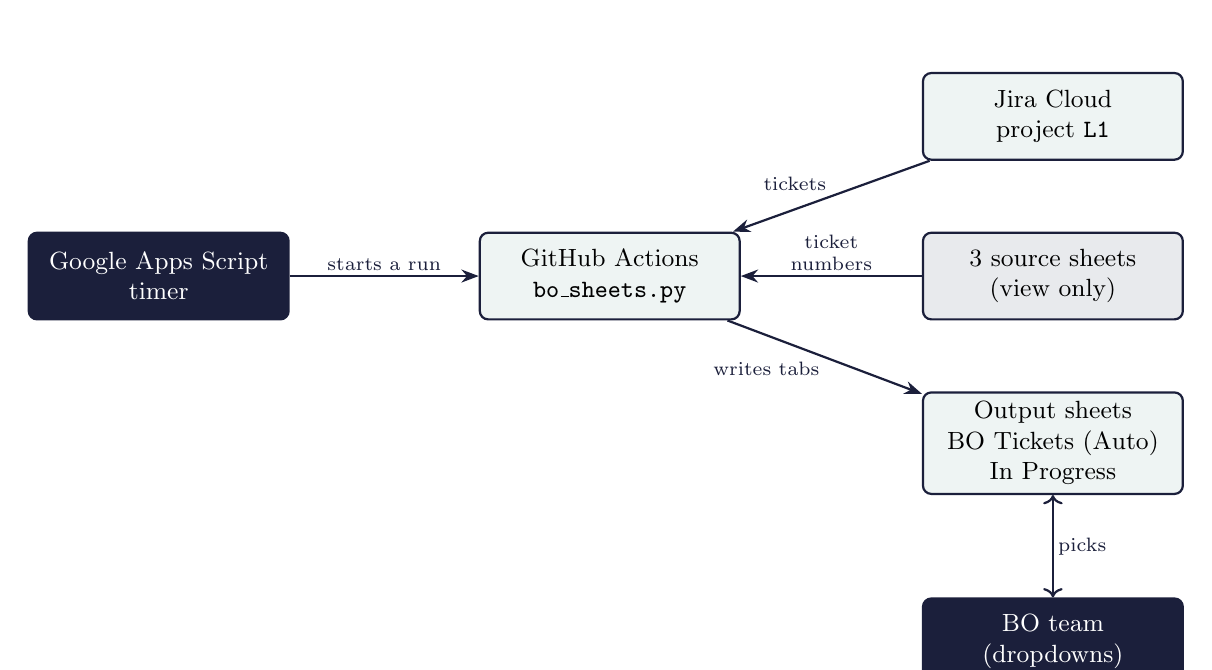
\begin{tikzpicture}[
  node distance=1.2cm and 1.6cm,
  box/.style={rectangle,rounded corners=3pt,draw=navy,fill=soft,thick,align=center,minimum width=3.3cm,minimum height=1.1cm,font=\small},
  dark/.style={box,fill=navy,text=white,draw=navy},
  src/.style={box,fill=sheetgrey},
  arr/.style={-{Stealth[length=2.2mm]},thick,color=navy},
  lab/.style={font=\scriptsize,align=center,fill=white,inner sep=1.5pt}]
  \node[dark] (timer) {Google Apps Script\\timer};
  \node[box,right=2.4cm of timer] (gh) {GitHub Actions\\\code{bo\_sheets.py}};
  \node[box,above right=0.9cm and 2.3cm of gh] (jira) {Jira Cloud\\project \code{L1}};
  \node[src,right=2.3cm of gh] (srcs) {3 source sheets\\(view only)};
  \node[box,below right=0.9cm and 2.3cm of gh] (out) {Output sheets\\BO Tickets (Auto)\\In Progress};
  \node[dark,below=1.3cm of out] (team) {BO team\\(dropdowns)};
  \draw[arr] (timer) -- node[lab,above]{starts a run} (gh);
  \draw[arr] (jira) -- node[lab,above left]{tickets} (gh);
  \draw[arr] (srcs) -- node[lab,above]{ticket\\numbers} (gh);
  \draw[arr] (gh) -- node[lab,below left]{writes tabs} (out);
  \draw[arr,<->] (team) -- node[lab,right]{picks} (out);
\end{tikzpicture}
\caption{How the parts connect. Arrows show the direction of data.}
\end{figure}

\subsection{Components}
\begin{tabularx}{\linewidth}{@{}l L@{}}
\toprule
\textbf{Component} & \textbf{Role} \\
\midrule
Jira Cloud (\code{connect-money.atlassian.net}) & Holds the tickets. Read only: the system never changes Jira. \\
\code{bo\_sheets.py} & The program. Reads Jira and the source sheets, builds the tabs, and writes them to Google
Sheets. \\
GitHub repository (private) & Stores the code and runs it on GitHub's servers through the workflow
\code{.github/workflows/sync.yml}. \\
Google Apps Script (\code{trigger.gs}) & A timer that asks GitHub to start a run at the right times. It does no data
work itself. \\
Google service account & A robot Google account that the program uses to read and write the sheets. \\
Output sheets & \tab{BO Tickets (Auto)} and \tab{In Progress}. Editable by the robot and the team. \\
Source sheets & Three existing team sheets that say which team a ticket belongs to. Read only. \\
\bottomrule
\end{tabularx}

\subsection{What happens in one refresh}
\begin{enumerate}
  \item The timer in Google Apps Script calls GitHub and starts the workflow.
  \item GitHub starts a small Linux machine, downloads the code, installs the Python libraries, and runs
    \code{bo\_sheets.py}.
  \item The program asks Jira for the relevant tickets, and at the same time reads the three source sheets.
  \item It decides which tab each ticket belongs to, and computes every column.
  \item It rewrites the tabs in both output sheets, keeping the dropdown choices people made, and rebuilds colours.
  \item The machine shuts down. A normal run takes about 30 seconds on GitHub (measured on 5 October 2026: 32 seconds).
\end{enumerate}

\begin{note}[Nothing is stored outside Google and GitHub]
The program keeps no database. Everything it needs to remember lives in the sheets themselves, including a hidden tab
called \tab{Done Log} (see Section~\ref{sec:donelog}).
\end{note}

% ================================================================ 3 DATA SOURCES
\section{Where the Data Comes From}

\subsection{Jira}
The program reads the Jira project \code{L1} (\emph{L1 Support (BO)}). It uses these ticket properties:

\begin{tabularx}{\linewidth}{@{}l L@{}}
\toprule
\textbf{Jira property} & \textbf{How it is used} \\
\midrule
Key (for example \code{L1-15393}) & Identifies the ticket; becomes a link in the sheet. \\
Status & Decides which sheet and tab the ticket appears in. \\
Assignee & Shown as the \tab{Person} in the In Progress sheet. \\
Created & Start of the ``days since arrived'' counter. \\
Request Type (L1) & The ``contact type''. Used for routing and for the Backlog table. \\
Summary & Contains the customer ticket reference at the end, for example \code{| CCS-15449}. \\
Status history (changelog) & Tells when a ticket entered its current status, and who closed it. \\
Related Tickets Status & Lists the linked tickets in other teams' projects and their status (used for \emph{With Team}). \\
\bottomrule
\end{tabularx}

\subsection{Jira statuses used}
\begin{tabularx}{\linewidth}{@{}l L@{}}
\toprule
\textbf{Meaning in the sheets} & \textbf{Jira statuses} \\
\midrule
\emph{New / untouched} & \code{To Do}, \code{Clients To Do} \\
\emph{In progress with BO} & \code{In Progress}, \code{Open}, \code{Reopened}, \code{Work in progress} \\
\emph{Waiting for the customer} & \code{Pending Customer Response} \\
\emph{Closed} & Every status Jira classifies as ``Done'' (for example \code{Done}, \code{Resolved BO},
\code{Resolved by OPS}, \code{Resolved by Collection}) \\
\emph{Everything else} & Pending with other teams (for example \code{Pending Tech (Lucky)}, \code{Pending BM});
treated as \emph{Pending} in the Backlog table and not shown on the ticket tabs \\
\bottomrule
\end{tabularx}

\begin{warning}[Jira's Resolution field is not used]
In this Jira, tickets are closed by moving them to a Done-type status; the \emph{Resolution} field is empty. The system
therefore recognises closed tickets by their status, not by resolution.
\end{warning}

\subsection{The three source sheets}
The queues (MDB, Installment, Product) are \emph{not} fields in Jira. The team keeps them in three Google Sheets. The
system reads those sheets (view only) to learn which team a ticket belongs to.

\begin{tabularx}{\linewidth}{@{}l L L@{}}
\toprule
\textbf{Team tab} & \textbf{Source sheet} & \textbf{Tabs read} \\
\midrule
MDB & \emph{MDP 2025/2026} (the sheet called ``MDB'' by the team) & All tabs \\
Installment & \emph{Credit Sheet} & Only \emph{Callcenter Cases 2026 V2} \\
Product & \emph{FO/BO 2026 - 2027} & All tabs (it has one) \\
\bottomrule
\end{tabularx}

A ticket ``belongs'' to a source sheet when its ticket number appears in any cell of that sheet. The program recognises
the number formats \code{L1-1234}, \code{CCS-1234}, \code{CC-1234}, and \code{CC2-1234}, and compares both the Jira key
and the customer reference from the summary. Cells longer than 40 characters are ignored, so a number mentioned inside a
long comment does not count.

% ================================================================ 4 BO SHEET
\section{The BO Tickets (Auto) Sheet}

\subsection{Which tickets appear}
Only tickets that satisfy \emph{all} of these:
\begin{itemize}
  \item They are in the Jira project \code{L1}.
  \item Their status is \code{To Do} or \code{Clients To Do}.
  \item They were created on or after \textbf{1 October 2026}.
\end{itemize}
When a ticket is picked up and its Jira status changes (for example to \emph{In Progress}), it disappears from this
sheet at the next refresh and appears in the \tab{In Progress} sheet instead.

\subsection{Tabs}
\begin{tabularx}{\linewidth}{@{}l L@{}}
\toprule
\textbf{Tab} & \textbf{Content} \\
\midrule
\tab{Backlog} & Closed / Pending / Untouched counts for each contact type (Section~\ref{sec:backlog}). \\
\tab{Productivity} & Live counts per team and per person (Section~\ref{sec:boprod}). \\
\tab{MDB} & To-do tickets that belong to the MDB team. \\
\tab{Installment} & To-do tickets that belong to the Installment team. \\
\tab{Product} & To-do tickets that belong to the Product team. \\
\tab{Others} & To-do tickets that match no team. Check it regularly. \\
\bottomrule
\end{tabularx}

\subsection{Columns of the ticket tabs}
\begin{tabularx}{\linewidth}{@{}l L@{}}
\toprule
\textbf{Column} & \textbf{Meaning} \\
\midrule
Key & The Jira ticket number. \\
Link & Opens the ticket in Jira. \\
Request Type & The contact type, as set in Jira. \\
Customer Ticket & The customer support reference taken from the end of the summary (for example \code{CCS-15449}). \\
Status & The Jira status (\emph{To Do} or \emph{Clients To Do}). \\
Assignee & \textbf{Dropdown} with the team names. Chosen by hand in the sheet. Not connected to Jira. \\
Created & When the ticket was created in Jira. \\
Updated & When the ticket was last changed in Jira (any comment, field change, or status change). \\
Resolved & \textbf{Dropdown}: \emph{Solved}, \emph{Pending for customer response}, \emph{On hold}. Chosen by hand. \\
\bottomrule
\end{tabularx}

The Summary column is deliberately not shown on this sheet.

\subsection{Extra columns copied from the source sheets}
\label{sec:extra}
To the right of \emph{Resolved}, each tab gets columns that the program copies from the team's source sheet. The row
is found by the ticket number, as in Section~\ref{sec:routing}.

\begin{tabularx}{\linewidth}{@{}l L@{}}
\toprule
\textbf{Tab} & \textbf{Columns added (and where they come from)} \\
\midrule
\tab{MDB} & \emph{Card \#}, \emph{Acc No}, \emph{Description}, \emph{Amount}, \emph{Disputed Amount If Partial},
\emph{Project}, \emph{BO Owner}, \emph{Validation}: the same-named columns of the MDP sheet. \\
\tab{Installment} & \emph{Comment}: the \emph{First Comment} column of the Credit Sheet. \\
\tab{Product} & \emph{Comment}: the \emph{Comment} column of the FO/BO sheet (often an escalation ticket such as
\code{TEC-14867}). \\
\tab{Others} & \emph{Comment}: no source sheet, so it starts empty and can be typed by hand. \\
\bottomrule
\end{tabularx}

\begin{itemize}
  \item A new ticket usually is not in the source sheet yet, because people fill those sheets by hand. Its cells stay
    empty and fill in automatically at the first refresh after the row appears.
  \item A \emph{Comment} typed by hand in this sheet is kept as long as the source sheet has no comment for that ticket.
    When the source sheet does have one, the source wins and replaces what was typed.
  \item \emph{Card \#} and \emph{Acc No} are stored as text, so numbers such as \code{0538} keep their leading zero.
\end{itemize}

\subsection{The dropdowns}
\begin{description}[leftmargin=!,labelwidth=3.4cm]
  \item[Assignee] Mego, Helana, Abdallah, Heba, Reem, Samy, Bassem, Mayar. The names are used exactly as written; the
    system never tries to match them to Jira users. The column starts empty.
  \item[Resolved] \swatch{sheetgreen}~Solved \quad \swatch{sheetyellow}~Pending for customer response \quad
    \swatch{sheetred}~On hold.
\end{description}
Each choice is coloured so the sheet can be scanned quickly. Choices are remembered by ticket key: when the sheet
refreshes, a choice stays with its ticket even if the ticket moves to a different tab.

\begin{warning}[Dropdown choices are only in the sheet]
Choosing \emph{Solved} here does \textbf{not} change the ticket in Jira. It is a working note for the team. Once the
ticket leaves the To Do list in Jira, it leaves this sheet and its choices go with it.
\end{warning}

\subsection{How a ticket is routed to a tab}
\label{sec:routing}
For every ticket the program follows the same three steps, in this order, and uses the first one that matches:
\begin{enumerate}
  \item \textbf{Keywords in the Request Type.} If the Request Type contains one of the words below, the ticket goes to
    that tab. The comparison ignores capital letters.
  \item \textbf{The source sheets.} If the ticket number is found in the MDB, then Installment, then Product source
    sheet, it goes to that tab.
  \item \textbf{Others.} Anything else.
\end{enumerate}

\begin{tabularx}{\linewidth}{@{}l L@{}}
\toprule
\textbf{Tab} & \textbf{Keywords (a Request Type containing any of these)} \\
\midrule
Installment & \code{installment}, \code{unable to pay due} \\
MDB & \code{refund transaction}, \code{purchase failed}, \code{deposit didn't reflect}, \code{pos transfer},
\code{unable to deposit}, \code{unable to withdraw} \\
Product & \code{different balance} \\
\bottomrule
\end{tabularx}

\begin{note}[Why keywords come first]
New tickets are often not yet written in the source sheets, because those sheets are filled in by hand. Keywords let
the system route a new ticket immediately. The source sheets are the fallback for types that no keyword covers.
\end{note}

\subsection{The Backlog tab}
\label{sec:backlog}
The table is modelled on the backlog table in the team's reporting. It covers \emph{every} ticket created since
1 October 2026 (not only the To Do ones), grouped by Request Type (the contact type), and sorted by the largest
\emph{Closed} count first.

\begin{tabularx}{\linewidth}{@{}l L@{}}
\toprule
\textbf{Column} & \textbf{Counts the tickets whose\ldots} \\
\midrule
\swatch{sheetgreen} Closed & status is a Done-type status. \\
\swatch{sheetyellow} Pending & status is anything else that is not To Do or Clients To Do. \\
\swatch{sheetred} Untouched & status is \code{To Do} or \code{Clients To Do} (nobody has started). \\
Total & is the sum of the three. \\
\bottomrule
\end{tabularx}
Each of the first three columns is shaded from white to a stronger colour: the darker the cell, the larger the number.
Use \textbf{Untouched} and \textbf{Pending} to see where the backlog is building up.

\subsection{The Productivity tab (BO sheet)}
\label{sec:boprod}
This tab is made of \textbf{live formulas} that read the other tabs, so the numbers change the moment someone changes a
dropdown, without waiting for a refresh.

\textbf{Left table: per team.} One row each for MDB, Installment, Product and Others, and a Total row.
\begin{itemize}
  \item \textbf{Total Tickets}: how many tickets are in that team's tab.
  \item \textbf{Solved}, \textbf{Pending for customer response}, \textbf{On hold}: how many tickets have that
    \emph{Resolved} choice.
  \item \textbf{Not Set Yet}: tickets with no \emph{Resolved} choice (total minus the three above).
\end{itemize}
\textbf{Right table: per person.} One row for each name in the Assignee dropdown, showing how many tickets that person
has in MDB, Installment, Product and Others, and a Total. The last row, \textbf{No one picked yet}, counts tickets that
have no Assignee choice.

% ================================================================ 5 IN PROGRESS SHEET
\section{The In Progress Sheet}

\subsection{Tabs}
\begin{tabularx}{\linewidth}{@{}l L@{}}
\toprule
\textbf{Tab} & \textbf{Content} \\
\midrule
\tab{MDB}, \tab{Installment}, \tab{Product}, \tab{Others} & Tickets currently in progress with the BO team, routed by the
same rules as the BO sheet (Section~\ref{sec:routing}). \\
\tab{Pending Customer Response} & Tickets sent back to the customer, with how long they have been waiting. \\
\tab{Productivity} & One row per person with their counts (Section~\ref{sec:ipprod}). \\
\emph{Done Log} (hidden) & The memory of who closed which ticket (Section~\ref{sec:donelog}). \\
\bottomrule
\end{tabularx}

\subsection{Which tickets appear and who is left out}
\label{sec:excluded}
\begin{itemize}
  \item Tickets whose Jira status is \code{In Progress}, \code{Open}, \code{Reopened}, or \code{Work in progress}
    appear on the team tabs, with no limit on age. A ticket stuck for a month still shows.
  \item Tickets in \code{Pending Customer Response} appear on their own tab.
  \item Tickets assigned to the following people are \textbf{left out of the whole sheet}: \emph{loay.khaled},
    \emph{nourhan.khaled}, \emph{mohanad.maher}, and \emph{Abdullah Mubark}.
  \item Unassigned tickets are shown with the person \emph{Unassigned}.
\end{itemize}

\subsection{Columns of the team tabs}
\begin{tabularx}{\linewidth}{@{}l L@{}}
\toprule
\textbf{Column} & \textbf{Meaning} \\
\midrule
Key, Link, Request Type, Summary & Ticket number, link to Jira, contact type, and the ticket summary. \\
Person & The Jira assignee. \\
Status & \textbf{Dropdown}: \swatch{sheetblue}~\emph{In Progress} or \swatch{sheetgreen}~\emph{Done}. The
team sets it by hand. New tickets start as In Progress. \\
Jira Status & The real status in Jira. \\
In Status Since & When the ticket entered its current Jira status. \\
Hours & Live counter: hours since ``In Status Since''. \\
Created & When the ticket was created. \\
Days Since Arrived & Live counter: days since ``Created''. \\
Days In Progress & Live counter: days since ``In Status Since''. \\
With Team & Which team has the problem now (Section~\ref{sec:withteam}). \\
Related Tickets (Jira) & The linked tickets in other teams' Jira projects and their status, as Jira lists them. \\
\bottomrule
\end{tabularx}

\begin{note}[How the live counters work]
\emph{Hours}, \emph{Days Since Arrived} and \emph{Days In Progress} are spreadsheet formulas based on the current
time. They keep increasing between refreshes without any help from the program. A ticket created at 09:00 shows
``0.5'' days at 21:00.
\end{note}

\subsection{Which team has the problem}
\label{sec:withteam}
Jira keeps a field called \emph{Related Tickets Status}. When a BO ticket is escalated, the field lists the linked ticket
in the other team's project and that ticket's status, for example
\code{Operations (OPS-1934): Pending CS}. The program reads this field and fills two columns on every ticket tab of the
In Progress sheet:
\begin{itemize}
  \item \textbf{Related Tickets (Jira)}: exactly what Jira lists, shortened to \emph{team, ticket, status}.
  \item \textbf{With Team}: who has the problem now, worked out with this rule:
\end{itemize}
\begin{tabularx}{\linewidth}{@{}L L@{}}
\toprule
\textbf{What Jira shows} & \textbf{With Team} \\
\midrule
No related ticket & \emph{BO} (or \emph{Customer} on the Pending Customer Response tab) \\
A related ticket whose status does \emph{not} mention CS, for example \emph{In Progress (OPS)} & the name of that
team, for example \emph{Operations} \\
Every related ticket has a CS status, for example \emph{Pending CS} or \emph{PENDING RESPONSE (CS)} &
\emph{BO (reply from Operations)}: the other team has answered and is waiting for us \\
\bottomrule
\end{tabularx}

\begin{warning}[This rule is an interpretation]
\emph{With Team} is based on the status wording ``CS'' meaning that the other team is waiting for Customer Support. If
the other teams use their statuses differently, the rule can be changed in one place in the program. The column
\emph{Related Tickets (Jira)} always shows the raw facts so the result can be checked.
\end{warning}
Tickets that sit in an escalation status of their own (for example \emph{Pending Tech (Lucky)} or \emph{Pending
Collection}) are not shown on this sheet; those statuses already name the team.

\subsection{The Status dropdown and what ``Done'' means}
\begin{itemize}
  \item The program does \textbf{not} add finished tickets to the team tabs automatically. A ticket finished in Jira
    simply leaves the tab.
  \item Instead, the team can mark a ticket \emph{Done} by hand while it is still open in Jira. The choice is kept
    through refreshes, and the ticket is counted as Done in the Productivity tab and in the tab's counters.
  \item Setting \emph{Done} does not change Jira. When the ticket is closed in Jira, it leaves the tab.
\end{itemize}

\subsection{Counters in the header row}
The top row of each tab also shows live totals, to the right of the table, so they are always visible:
\begin{itemize}
  \item Team tabs: \textbf{Total}, \textbf{In Progress}, and \textbf{Done} (based on the Status dropdown).
  \item Pending Customer Response: \textbf{Total} and \textbf{Overdue}.
  \item Productivity: \textbf{All people} (the grand total of cases).
\end{itemize}
The filter arrows cover only the ticket columns, so sorting or filtering a table never moves the counters.

\subsection{The Pending Customer Response tab}
Lists the tickets in the Jira status \emph{Pending Customer Response}. It has the same columns as the team tabs, with
these differences:
\begin{itemize}
  \item \textbf{Sent To Customer} replaces ``In Status Since'': the time the ticket was put into that status.
  \item \textbf{Days Waiting For Customer} replaces ``Days In Progress''.
  \item \textbf{Over 48h?} shows \swatch{sheetred}~\textbf{OVERDUE} when the ticket has waited more than
    \textbf{48 hours}. This is the \emph{only} place in the sheet with an overdue flag. The team tabs have none.
\end{itemize}

\subsection{The Productivity tab (In Progress sheet)}
\label{sec:ipprod}
One row per person, listed once, largest total first. Colours work like the Backlog table.

\begin{tabularx}{\linewidth}{@{}l L@{}}
\toprule
\textbf{Column} & \textbf{Meaning} \\
\midrule
Person & The person's Jira name. \\
In Progress & Their open tickets whose Status dropdown is not \emph{Done}. \\
Done (last 30 days) & Tickets they moved to a Done-type status in Jira in the last 30 days, plus open tickets they
have marked \emph{Done} in the sheet. \\
Pending Customer & Their tickets that are waiting for the customer. \\
Total Cases & In Progress + Done + Pending Customer. \\
\bottomrule
\end{tabularx}

\begin{warning}[How to read the Done numbers]
``Done'' is credited to the person who \emph{moved the ticket} to the Done status in Jira, which may differ from the
assignee. If someone closes a large batch of old tickets at once, their number jumps. Read large numbers together with
the dates, and do not use them as a measure of individual speed without checking.
\end{warning}
The excluded people (Section~\ref{sec:excluded}) do not appear. Tickets with no assignee are not listed in Productivity, because they
belong to nobody.

\subsection{The hidden Done Log tab}
\label{sec:donelog}
Reading the full Jira history of about 3\,200 recently closed tickets takes over 30 seconds, which is too slow to do
every run. Instead, the program keeps a hidden tab named \tab{Done Log} with one row per closed ticket: its key, the
time it was closed (as a Unix time in seconds), and who closed it. A cell beside it records the time of the last run.
Each refresh only asks Jira about tickets that changed since then, adds them, removes tickets that were reopened, and
drops entries older than 30 days.

\begin{warning}[Do not delete or edit the Done Log]
If it is deleted, nothing breaks: the next run rebuilds it from the last 30 days, which takes about 40 seconds once.
Editing it by hand will change the Done counts.
\end{warning}

\subsection{Colour guide}
\begin{tabularx}{\linewidth}{@{}l L@{}}
\toprule
\textbf{Colour} & \textbf{Where and what it means} \\
\midrule
\swatch{sheetgreen} Green & \emph{Done}, \emph{Solved}, and the Closed column. \\
\swatch{sheetblue} Blue & \emph{In Progress}. \\
\swatch{sheetyellow} Yellow & \emph{Pending Customer Response}, \emph{Pending for customer response}, and Pending columns. \\
\swatch{sheetred} Red & \emph{On hold}, \emph{Reopened}, the Untouched column, and \textbf{OVERDUE}. \\
\swatch{sheetgrey} Grey & \emph{To Do}. \\
\swatch{sheetpurple} Purple & \emph{Clients To Do}. \\
\bottomrule
\end{tabularx}

% ================================================================ 6 AUTOMATION
\section{How the Sheets Stay Up to Date}

\subsection{When a refresh happens}
A Google Apps Script timer wakes up every 30 minutes and decides whether to start a run:
\begin{center}
\begin{tabular}{@{}ll@{}}
\toprule
\textbf{Time (Cairo)} & \textbf{Refresh} \\
\midrule
09:00 -- 22:59 (day) & every 30 minutes (about 28 runs) \\
23:00 -- 08:59 (night) & every 2 hours: 23:00, 01:00, 03:00, 05:00, 07:00 (5 runs) \\
\bottomrule
\end{tabular}
\end{center}
Google's timer handles the clock change at the end of October (Egypt moves from UTC+3 to UTC+2) automatically, so the
schedule needs no edit. A refresh can also be started by hand (Section~\ref{sec:manual}).

\subsection{What a refresh changes}
\begin{itemize}
  \item Every tab is cleared and rewritten from fresh data.
  \item \textbf{Kept:} the team's dropdown choices (Assignee, Resolved, Status), matched by ticket key.
  \item \textbf{Rebuilt:} colours, dropdown lists, and the order of tabs.
  \item \textbf{Live:} all counters and totals are formulas, so they update by themselves.
\end{itemize}
If someone picks a dropdown value at the very second a refresh finishes, the choice can occasionally be lost. Check that
it stuck.

\subsection{Running time and free minutes}
\label{sec:minutes}
GitHub's free plan for private repositories includes \textbf{2\,000 minutes per month}, and each run is rounded up to
whole minutes.

\begin{center}
\begin{tabular}{@{}lr@{}}
\toprule
Runs per day (28 day + 5 night) & 33 \\
Runs per month (30 days) & about 990 \\
Billed minutes if each run is under 1 minute & about 990 \\
Billed minutes if each run takes 1--2 minutes & about 1\,980 \\
Free allowance & 2\,000 \\
\bottomrule
\end{tabular}
\end{center}
A normal run was measured at 32 seconds, so the expected use is about 1\,000 minutes a month, with a safety margin.
Check \emph{Settings $\rightarrow$ Billing $\rightarrow$ Actions} on GitHub from time to time.

\subsection{Why the timer lives in Google and not in GitHub}
GitHub can start workflows on a schedule of its own, and this was the first design. In practice GitHub's scheduler is
\emph{best effort}: on the first day it started only one scheduled run over more than six hours, so new tickets did not
reach the sheet. The Google timer does not have this problem. The GitHub schedule was therefore removed, and the
workflow now runs only when called by the Google timer or by hand.

\subsection{Starting a refresh by hand}
\label{sec:manual}
Open the repository on GitHub, choose the \textbf{Actions} tab, select \textbf{Sync Jira to Google Sheets}, and click
\textbf{Run workflow}. The run appears in the list and finishes in about 30 seconds.

% ================================================================ 7 SETUP
\section{Setup and Configuration (for the Maintainer)}

\subsection{Repository contents}
\begin{tabularx}{\linewidth}{@{}l L@{}}
\toprule
\textbf{File} & \textbf{Purpose} \\
\midrule
\code{bo\_sheets.py} & The main program (both sheets). \\
\code{jira\_to\_sheets.py} & The first, simpler exporter (one flat table). No longer used by the workflow. \\
\code{requirements.txt} & Python libraries: \code{requests}, \code{gspread}, \code{google-auth}. \\
\code{.github/workflows/sync.yml} & The workflow that runs the program. \\
\code{apps-script/trigger.gs} & The Google timer code. \\
\code{.env.example} & List of all settings, without secrets. \\
\code{docs/} & This document and the logo files. \\
\bottomrule
\end{tabularx}

\subsection{Settings}
Settings are environment variables. In the workflow, secrets come from GitHub's secret store and the rest are written in
the workflow file.

\begin{longtable}{@{}p{5.5cm} p{3.0cm} p{5.7cm}@{}}
\toprule
\textbf{Setting} & \textbf{Default} & \textbf{Meaning} \\
\midrule
\endhead
\code{JIRA\_BASE\_URL} & (set in workflow) & Jira site address. \\
\code{JIRA\_EMAIL} & (set in workflow) & Login email used with the Jira token. \\
\code{JIRA\_API\_TOKEN} & \textbf{secret} & Jira API token. \\
\code{GOOGLE\_SERVICE\_\allowbreak ACCOUNT\_JSON} & \textbf{secret} & Full contents of the service account key. \\
\code{BO\_SHEET\_ID} & (set in workflow) & Spreadsheet ID of BO Tickets (Auto). \\
\code{INPROGRESS\_SHEET\_ID} & (set in workflow) & Spreadsheet ID of In Progress. \\
\code{JIRA\_PROJECT} & \code{L1} & Jira project key. \\
\code{BO\_FROM} & \code{2026-10-01} & BO sheet shows tickets created on or after this date. \\
\code{BO\_TODO\_STATUSES} & To Do, Clients To Do & Statuses that count as untouched. \\
\code{INPROGRESS\_STATUSES} & In Progress, Open, Reopened, Work in progress & Statuses shown as in progress. \\
\code{CUSTOMER\_STATUS} & Pending Customer Response & Status for the customer-waiting tab. \\
\code{PENDING\_SLA\_HOURS} & 48 & Hours before a customer-waiting ticket is OVERDUE. \\
\code{PRODUCTIVITY\_DAYS} & 30 & Window for the Done counts. \\
\code{EXCLUDED\_PEOPLE} & loay.khaled, nourhan.khaled, mohanad.maher, Abdullah Mubark & Left out of the In Progress sheet. \\
\code{SHEET\_TIMEZONE} & \code{Africa/Cairo} & Time zone set on both sheets. \\
\code{MDB\_SOURCE\_ID}, \code{INSTALLMENT\_\allowbreak SOURCE\_ID}, \code{INSTALLMENT\_\allowbreak SOURCE\_TAB}, \code{PRODUCT\_SOURCE\_ID} & the three source sheets & Where the team sheets are. \\
\bottomrule
\end{longtable}

\subsection{Building it from scratch}
\begin{enumerate}
  \item \textbf{Jira token.} At \url{https://id.atlassian.com/manage-profile/security/api-tokens} create an API token for
    the Jira account. Choose an expiry date.
  \item \textbf{Google project.} In Google Cloud Console, enable the \emph{Google Sheets API} (and the \emph{Google
    Drive API}). Create a \emph{service account} and download its JSON key.
  \item \textbf{Create the two output sheets} in a normal Google account (a service account has no storage of its own
    and cannot create files). Share both with the service account's email address as \textbf{Editor}.
  \item \textbf{Share the three source sheets} with the same address as \textbf{Viewer}.
  \item \textbf{GitHub.} Keep the repository \textbf{private}. Under \emph{Settings $\rightarrow$ Secrets and variables
    $\rightarrow$ Actions} add the secrets \code{JIRA\_API\_TOKEN} and \code{GOOGLE\_SERVICE\_ACCOUNT\_JSON} (paste the
    whole key file, from the first \code{\{} to the last \code{\}}, brackets included).
  \item \textbf{GitHub access token for the timer.} Create a fine-grained personal access token limited to this one
    repository with only \emph{Actions: Read and write}. Choose an expiry date and note it.
  \item \textbf{Google timer.} In the BO sheet open \emph{Extensions $\rightarrow$ Apps Script}, paste the code from
    Appendix~\ref{app:script}, and save. In \emph{Project Settings $\rightarrow$ Script properties} add
    \code{GITHUB\_TOKEN} with the token from step 6. Run \code{triggerSync} once and accept the permission request.
    Under \emph{Triggers} add a time-driven trigger for \code{triggerSync}, minutes timer, every 30 minutes.
  \item \textbf{Check.} The Actions tab should show a new run, and the sheets should fill.
\end{enumerate}

\begin{warning}[Two expiry dates to track]
The Jira token and the GitHub token both expire. The GitHub token used for the timer expires on \textbf{4 November
2026}. After expiry the timer fails quietly and the sheets stop updating. Create a new token before that date, and paste
it into the Apps Script property \code{GITHUB\_TOKEN}.
\end{warning}

% ================================================================ 8 HOW TO CHANGE
\section{Everyday Maintenance}

\begin{longtable}{@{}p{4.9cm} p{9.3cm}@{}}
\toprule
\textbf{I want to\ldots} & \textbf{Do this} \\
\midrule
\endhead
Send a new kind of ticket to a tab & Add a keyword to \code{KEYWORDS} in \code{bo\_sheets.py} (Section~\ref{sec:routing}),
or add the ticket numbers to the matching source sheet. \\
Check which tickets are in \emph{Others} & Open the Others tab, read the \emph{Request Type} column, and decide which
tab each type belongs to. Then add a keyword for it. \\
Add or remove a name in the Assignee dropdown & Edit the list \code{TEAM} in \code{bo\_sheets.py}. \\
Leave another person out of the In Progress sheet & Add their Jira display name to \code{EXCLUDED\_PEOPLE}. \\
Change the 48-hour limit & Set \code{PENDING\_SLA\_HOURS}. \\
Change the BO sheet's start date & Set \code{BO\_FROM} (format \code{YYYY-MM-DD}). \\
Count other statuses as in progress & Set \code{INPROGRESS\_STATUSES}. \\
Change how often it refreshes & Edit the day and night rules in the Apps Script (Appendix~\ref{app:script}); mind the
free minutes (Section~\ref{sec:minutes}). \\
Refresh now & Run the workflow by hand (Section~\ref{sec:manual}). \\
Rebuild the Done counts & Delete the hidden \emph{Done Log} tab; the next run rebuilds it. \\
Replace an expiring token & Create a new token and replace the secret (GitHub) or the property (Apps Script). \\
\bottomrule
\end{longtable}

\noindent All code changes go through the repository: edit the file, commit to a working branch, and merge into
\code{main}. The workflow always runs the code on \code{main}.

% ================================================================ 9 TROUBLESHOOTING
\section{Troubleshooting}

\begin{longtable}{@{}p{4.4cm} p{4.5cm} p{5.3cm}@{}}
\toprule
\textbf{What you see} & \textbf{Likely cause} & \textbf{What to do} \\
\midrule
\endhead
Sheet is hours old, new tickets missing & The timer did not start a run, or the run failed. &
Look at the repository's Actions tab. If there are no recent runs, check the Apps Script \emph{Executions} list. Start a
run by hand. \\
Apps Script error \code{404} & The GitHub token cannot see the private repository. &
Check that the token's owner and repository are right and that \emph{Actions: Read and write} is set. \\
Apps Script error \code{401} / \code{403} & Token wrong, expired, or lacking permission. & Create a new token. \\
Run fails with \code{429} & Google's limit on requests per minute. &
The program waits 70 seconds and retries up to four times. If it keeps failing, wait and run again. \\
A ticket is missing from the BO sheet & It is not To Do / Clients To Do, was created before 1 October 2026, or is in a
different project. & Check the ticket in Jira. \\
A ticket is in \emph{Others} & No keyword matches and it is not in a source sheet. & Add a keyword or add it to the
source sheet. \\
A dropdown choice vanished & The ticket left the list, or a refresh finished while it was chosen. &
Choose it again; check the ticket's Jira status. \\
Done numbers look too high & A person closed many tickets at once. & Check dates; see Section~\ref{sec:ipprod}. \\
Counters show an error & A tab was renamed, or a column moved. & Do not rename tabs or move columns; run a refresh to rebuild. \\
Run fails with a Jira error & Jira token expired or the Jira site is unavailable. & Create a new token, or wait. \\
\bottomrule
\end{longtable}

\begin{note}[The first place to look]
Open the \textbf{Actions} tab in the GitHub repository. Each run shows a green tick or a red cross. Click a red run to
read the exact error message.
\end{note}

% ================================================================ 10 SECURITY
\section{Security and Data Handling}
\label{ch:security}

\begin{itemize}
  \item \textbf{Secrets are never in the code.} The repository holds no token or key. The Jira token and the Google key
    live in GitHub's encrypted secret store. The GitHub token lives in the Apps Script's script properties.
  \item \textbf{The repository must stay private.} It contains the sheet addresses and the company's Jira site name.
  \item \textbf{Least access.} The service account can edit only the two output sheets and can only view the three
    source sheets. The GitHub token can only start workflows in this one repository.
  \item \textbf{Read only on Jira.} The program never changes a ticket.
  \item \textbf{Sheet privacy.} Both output sheets are restricted: only people they are shared with can open them.
  \item \textbf{Personal data.} The sheets show ticket numbers, request types, summaries, and staff names. They do not
    copy customer phone numbers or card details from the source sheets: the source sheets are read only to find ticket
    numbers.
\end{itemize}

\begin{warning}[Rotate credentials that were shared during development]
During development, a Jira token and a service account key were pasted into a chat session. A credential that has been
shared should be treated as exposed. Revoke those tokens (Jira: \emph{Security $\rightarrow$ API tokens}; Google Cloud:
delete and re-create the service account key) and put the new values only into the GitHub secrets.
\end{warning}

% ================================================================ 11 LIMITS
\section{Limits, Decisions, and Open Items}

\subsection{Decisions made along the way}
\begin{itemize}
  \item \textbf{Keywords before source sheets.} Routing by Request Type keywords gives instant results for new
    tickets; the hand-filled source sheets are the fallback.
  \item \textbf{Names used as given.} The Assignee dropdown is never matched to Jira users.
  \item \textbf{Done is a manual dropdown.} The In Progress tabs do not list finished tickets automatically.
  \item \textbf{Overdue only for customer waiting.} The 24-hour overdue flag was removed from the team tabs; the
    customer-waiting tab uses 48 hours.
  \item \textbf{One timer.} Only the Google timer starts runs, so refreshes are not doubled.
\end{itemize}

\subsection{Known limits}
\begin{itemize}
  \item The sheets can be up to 30 minutes behind Jira by day and about 2 hours behind overnight.
  \item Dropdown choices do not write back to Jira.
  \item Done is credited to the person who moved the ticket, so batch closures distort individual numbers.
  \item Some tickets have no assignee in Jira (about 80 at the time of writing); they appear as \emph{Unassigned} on the team tabs and are left out of
    Productivity.
  \item The Others tab depends on the keyword list; new request types land there until a keyword is added.
  \item The team has not yet decided where some request types belong (for example \emph{Card is temporarily blocked}
    and \emph{Credit Limit Not Activated}); they currently fall under Others on the In Progress sheet.
  \item Google allows about 60 reads and 60 writes per minute for this service account. A normal run uses far fewer.
\end{itemize}

\subsection{Open items}
\begin{enumerate}
  \item Decide the team for the request types that currently land in \emph{Others}.
  \item Decide whether the In Progress sheet should also get the Backlog table, the Assignee dropdown, or the Resolved
    dropdown, as on the BO sheet.
  \item Replace the GitHub token before 4 November 2026.
  \item Review the monthly free-minute usage in mid-month and at the end of the month.
  \item Revoke and replace the credentials that were shared during development (Chapter~\ref{ch:security}).
\end{enumerate}

% ================================================================ 12 WALKTHROUGH
\section{A Ticket's Journey: Putting It Together}
\begin{enumerate}
  \item \textbf{A customer contacts support.} A Jira ticket is created in project \code{L1} with status \emph{To Do}.
  \item \textbf{Within 30 minutes} (or 2 hours overnight) the ticket appears in the \textbf{BO Tickets (Auto)} sheet, in
    the tab chosen by its Request Type (for example \emph{Lucky Refund Transaction} $\rightarrow$ \tab{MDB}). It counts as
    \emph{Untouched} in the Backlog tab.
  \item \textbf{Someone takes it.} In the sheet they pick their name under \emph{Assignee}, and the per-person table in
    Productivity moves by one. In Jira the ticket moves to \emph{In Progress}.
  \item \textbf{At the next refresh} the ticket leaves the BO sheet and appears in the \textbf{In Progress} sheet, on the
    team tab, with a live \emph{Hours} and \emph{Days} counter. Backlog now counts it as \emph{Pending}.
  \item \textbf{The team asks the customer for information.} In Jira the status becomes \emph{Pending Customer
    Response}. The ticket moves to that tab; after 48 hours it shows \textbf{OVERDUE}.
  \item \textbf{The ticket is closed in Jira} (for example \emph{Resolved BO}). It leaves the In Progress sheet, is
    written to the Done Log with the name of whoever closed it, and counts toward that person's \emph{Done} for the next
    30 days. Backlog counts it as \emph{Closed}.
\end{enumerate}

% ================================================================ 13 HISTORY
\section{Project History}
\begin{tabularx}{\linewidth}{@{}l L@{}}
\toprule
\textbf{Step} & \textbf{What was built} \\
\midrule
1 & First exporter: all Jira tickets into one private Google Sheet. \\
2 & Connection to Jira and Google verified; service account sharing set up. \\
3 & BO sheet and In Progress sheet created, with Pending Customer Response and Productivity. \\
4 & Routing into MDB, Installment, Product; Others tab; source sheets read for matching. \\
5 & Dropdowns (Assignee, Resolved) with colours; Summary and Reporter columns removed. \\
6 & Automatic refresh with GitHub Actions; schedule tuned to working hours and the free minutes. \\
7 & In Progress sheet reorganised into team tabs; Status dropdown; 48-hour customer flag; one-row-per-person
productivity; Backlog table. \\
8 & Day counters (days since arrived, days in progress). \\
9 & Reliability fix: GitHub's scheduler skipped runs, so the Google timer now starts every run. \\
10 & Speed-up: Done Log, parallel reads, batched writes (run time from about 80 seconds to about 30 seconds). \\
11 & BO Productivity tab; live totals in the In Progress tabs; this document. \\
12 & MDP case columns on the BO MDB tab; Comment column on the other BO tabs; \emph{With Team} and \emph{Related Tickets}
on the In Progress sheet. \\
\bottomrule
\end{tabularx}

\clearpage
% ================================================================ APPENDICES
\appendix

\section{Glossary}
\begin{description}[leftmargin=!,labelwidth=3.6cm]
  \item[BO] Back Office, the team this system serves.
  \item[L1] The key of the Jira project \emph{L1 Support (BO)}.
  \item[MDB / MDP] The team's name for the queue that is tracked in the sheet \emph{MDP 2025/2026}.
  \item[Request Type] The Jira field that says what the customer contacted support about (also called the contact type).
  \item[Customer ticket (CCS)] The reference of the original customer support ticket; written at the end of a Jira
    summary.
  \item[Backlog] Work that has arrived but is not finished.
  \item[Untouched] A ticket nobody has started (status To Do or Clients To Do).
  \item[Pending] A ticket that is open but not untouched.
  \item[Overdue] A customer-waiting ticket that has waited more than 48 hours.
  \item[Workflow] A set of steps that GitHub runs on a server; here, the refresh.
  \item[Secret] A password or key stored encrypted so that nobody can read it back.
  \item[Service account] A robot Google account used by programs.
  \item[Apps Script] Google's built-in scripting tool for Google Sheets.
  \item[JQL] Jira's query language, used to ask Jira for a list of tickets.
  \item[Dropdown] A cell that lets you pick from a fixed list.
\end{description}

\section{Quick Checklists}
\subsection*{Every day (team lead)}
\begin{itemize}[label=$\square$]
  \item The \emph{Updated} column in the BO sheet shows recent times.
  \item The \emph{Others} tab is empty or understood.
  \item Pending Customer Response: any \textbf{OVERDUE} rows to chase.
\end{itemize}
\subsection*{Every week (maintainer)}
\begin{itemize}[label=$\square$]
  \item Latest runs in the Actions tab are green and appear on schedule.
  \item Request types in \emph{Others} have been assigned keywords.
\end{itemize}
\subsection*{Every month}
\begin{itemize}[label=$\square$]
  \item GitHub billing page: Actions minutes used are well under 2\,000.
  \item Token expiry dates (Jira, GitHub) are more than two weeks away.
\end{itemize}

\section{Google Apps Script (timer)}
\label{app:script}
This is the full code of the timer. It contains no secret: the token is read from the script property
\code{GITHUB\_TOKEN}.
\begin{lstlisting}[language=Java]
const REPO = 'mazenDDr/jira-magdy';
const WORKFLOW = 'sync.yml';
const BRANCH = 'main';
const TIME_ZONE = 'Africa/Cairo';

function triggerSync() {
  const now = new Date();
  const hour = Number(Utilities.formatDate(now, TIME_ZONE, 'H'));
  const minute = Number(Utilities.formatDate(now, TIME_ZONE, 'm'));
  const night = hour >= 23 || hour < 9;
  // overnight, only the first trigger of every second hour (odd hours: 23, 1, 3, 5, 7)
  if (night && (hour % 2 === 0 || minute >= 30)) return;

  const token = PropertiesService.getScriptProperties().getProperty('GITHUB_TOKEN');
  if (!token) throw new Error('Add GITHUB_TOKEN under Project Settings > Script properties');

  const response = UrlFetchApp.fetch(
    'https://api.github.com/repos/' + REPO + '/actions/workflows/' + WORKFLOW + '/dispatches',
    {
      method: 'post',
      contentType: 'application/json',
      headers: {
        Authorization: 'Bearer ' + token,
        Accept: 'application/vnd.github+json',
        'X-GitHub-Api-Version': '2022-11-28',
      },
      payload: JSON.stringify({ ref: BRANCH }),
      muteHttpExceptions: true,
    });
  if (response.getResponseCode() !== 204) {
    throw new Error('GitHub answered ' + response.getResponseCode() + ': ' + response.getContentText());
  }
}
\end{lstlisting}

\section{GitHub Workflow}
\label{app:workflow}
The file \code{.github/workflows/sync.yml}. The secrets are referenced by name only.
\begin{lstlisting}[language=bash]
name: Sync Jira to Google Sheets

on:
  # Started by the Google Apps Script timer or by hand from the Actions tab.
  workflow_dispatch:

concurrency:
  group: sync-sheets
  cancel-in-progress: false

jobs:
  sync:
    runs-on: ubuntu-latest
    timeout-minutes: 9
    steps:
      - uses: actions/checkout@v4
      - uses: actions/setup-python@v5
        with:
          python-version: "3.11"
          cache: pip
      - run: pip install -r requirements.txt
      - run: python bo_sheets.py
        env:
          JIRA_BASE_URL: https://connect-money.atlassian.net
          JIRA_EMAIL: <the Jira login email>
          JIRA_API_TOKEN: ${{ secrets.JIRA_API_TOKEN }}
          GOOGLE_SERVICE_ACCOUNT_JSON: ${{ secrets.GOOGLE_SERVICE_ACCOUNT_JSON }}
          BO_SHEET_ID: <id of BO Tickets (Auto)>
          INPROGRESS_SHEET_ID: <id of In Progress>
\end{lstlisting}
\noindent The \code{concurrency} setting makes sure two runs never write to the sheets at the same time: a second run
waits for the first.

\vfill
\begin{center}
\small\color{black!60} Prepared by \textbf{Mohamed Magdy} \quad$\cdot$\quad Connect Money \quad$\cdot$\quad October 2026
\end{center}

\end{document}
